\documentclass{beamer}
\usepackage[english]{babel}
\usepackage{../mathsutil}
\usepackage{../fdtdutil}
\usepackage{tikz}
\usetikzlibrary{fadings}
\usetikzlibrary{patterns}
\usetikzlibrary{shadows.blur}
\usetikzlibrary{shapes}
\usetikzlibrary{calc}
\usetheme{Madrid}
%Information to be included in the title page:
\title{Estudo Dirigido 1}
\author{Téssio Perotti Arruda}
\institute{UnB}
\date{2022}

\institute[UnB] % (optional)
{
  \inst{1}%
  Electrical Engineering\\
  University of Brasilia
}

\date[ED1 2022.1] % (optional)
{Estudo Dirigido 1 - Final Report, September 2022}

\logo{\includegraphics[height=0.75cm]{unb}}

\begin{document}


\frame{\titlepage}

\begin{frame}{Outline}
  \tableofcontents
\end{frame}

\AtBeginSection[ ]
{
\begin{frame}{Outline}
    \tableofcontents[currentsection]
\end{frame}
}

\section{Expansion of Maxwell's Curl Equations in Cartesian Coordinates}

\begin{frame}{Maxwell's Equations in Cartesian Coordinates}
The Maxwell's Equations are:
\begin{align*}
    \rot \Et(t) &= -\partial _t \Bt(t), \\
    \rot \Hht(t) &= \partial_t \Dt(t), \\
    \Div \Bt(t) &= 0, \\
    \Div \Dt(t) &= 0,
\end{align*}
where $\partial_t\cdot = \partialDerivative{\cdot}{t}$.
The the constitutive relations are:
\begin{align}
    \Bt(t) &= \brackets{\mu_0\mu_r  (t)} \ast \Hht(t), \\
    \Dt(t) &= \brackets{\epsilon_0 \epsilon_r  (t)} \ast \Et(t),
\end{align}
where $\brackets{\cdot}$ represents a tensor.
\end{frame}


\begin{frame}{Normalizing the Electric Fields}
  It will be adopted the conventional approach in FDTD and the electric field will be normalized as:
  \begin{equation}
    \tilde{\Et}(t) = \sqrt{\cfrac{\epsilon_0}{\mu_0}}\Et(t) = \cfrac{1}{\eta_0}\Et(t).
  \end{equation}

  The other parameters related to the electric field must also be normalized:
  \begin{equation}
      \tilde{\Dt} = \sqrt{\cfrac{1}{\epsilon_0\mu_0}} \Dt = c_0 \Dt.
  \end{equation}

\end{frame}

\begin{frame}{Normalized Maxwell's equations}
  Therefore, the normalized Maxwell's equations become:
  \begin{align}
      \rot \En &= -\partial _t \Bt, \\
      \rot \Hht &= \partial_t \Dn, \\
      \Div \Bt &= 0, \\
      \Div \Dn &= 0.
  \end{align}
\end{frame}


\begin{frame}{Expanding Maxwell's equations}
  To expand the equations, it will be assumed that $\brackets{\mu_r}$ and $\brackets{\epsilon_r}$ has only diagonal terms \cite{rumpf_book}. 
  \begin{columns}
    \begin{column}{0.45\textwidth}
      \begin{align}
        \partial_z\En_y - \partial_y\En_z &= \cfrac{\mu_{xx}}{c_0} \partial_t \Hht_x \\
        \partial_x\En_z - \partial_z\En_x &= \cfrac{\mu_{yy}}{c_0} \partial_t \Hht_y\\
        \partial_y\En_x - \partial_x\En_y &= \cfrac{\mu_{zz}}{c_0} \partial_t \Hht_z
      \end{align}
    \end{column}
    \begin{column}{0.45\textwidth}
      \begin{align}
        \partial_z\Hht_y - \partial_y\Hht_z &= \cfrac{1}{c_0} \partial_t \Dn_x \\
        \partial_x\Hht_z - \partial_z\Hht_x &= \cfrac{1}{c_0} \partial_t \Dn_y \\
        \partial_y\Hht_x - \partial_x\Hht_y &= \cfrac{1}{c_0} \partial_t \Dn_z
    \end{align}

    \end{column}

  \end{columns}

  \begin{align}
      \Dn_x &= \epsilon_{xx} \En_x \label{eq:Dn_x}\\
      \Dn_y &= \epsilon_{yy} \En_y \label{eq:Dn_y}\\
      \Dn_z &= \epsilon_{zz} \En_z \label{eq:Dn_z}
  \end{align}
\end{frame}


\begin{frame}{Notation for Curl Terms}

  \begin{align}
    \CEx &= \partial_z\En_y - \partial_y\En_z \\
    \CEy &= \partial_x\En_z - \partial_z\En_x \\
    \CEz &= \partial_y\En_x - \partial_x\En_y
  \end{align}

  \begin{align}
    \CHx &= \partial_z\Hht_y - \partial_y\Hht_z \\
    \CHy &= \partial_x\Hht_z - \partial_z\Hht_x \\
    \CHz &= \partial_y\Hht_x - \partial_x\Hht_y
  \end{align}

\end{frame}

\begin{frame}{Final Equations Form}
  \begin{columns}
    \begin{column}{0.45\textwidth}
      \begin{align}
        \CEx &= \cfrac{\mu_{xx}}{c_0} \partial_t \Hht_x \\
        \CEy &= \cfrac{\mu_{yy}}{c_0} \partial_t \Hht_y\\
        \CEz &= \cfrac{\mu_{zz}}{c_0} \partial_t \Hht_z
    \end{align}
    \end{column}
    \begin{column}{0.45\textwidth}
      \begin{align}
        \CHx &= \cfrac{1}{c_0} \partial_t \Dn_x \\
        \CHy &= \cfrac{1}{c_0} \partial_t \Dn_y \\
        \CHz &= \cfrac{1}{c_0} \partial_t \Dn_z
    \end{align}
    \end{column}

  \end{columns}

  \begin{align}
    \Dn_x &= \epsilon_{xx} \En_x \label{eq:dnx_update} \\
    \Dn_y &= \epsilon_{yy} \En_y \label{eq:dny_update} \\
    \Dn_z &= \epsilon_{zz} \En_z \label{eq:dnz_update}
\end{align}
\end{frame}

\begin{frame}{Yee Grid}
  
A unit cell is constructed by dividing the 3 axis into discrete cells of size $(\dx, \dy, \dz)$. Inside this cell, it is necessary to put all the fields of the electromagnetic problem $(\Et_x, \Et_y, \Et_z, \Hht_x, \Hht_x, \Hht_z)$. Instead of putting all fields on the origin $(0, 0, 0)$, where is more intuitive, Yee proposed the following approach:

\centering


\tikzset{every picture/.style={line width=0.75pt}} %set default line width to 0.75pt        

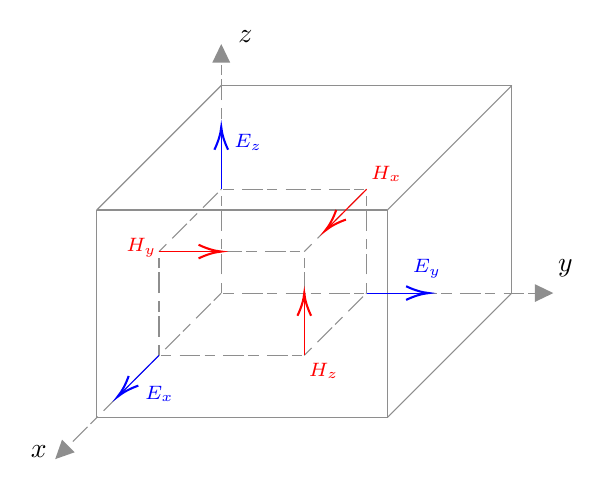
\begin{tikzpicture}[x=0.75pt,y=0.75pt,yscale=-1,xscale=1]
%uncomment if require: \path (0,300); %set diagram left start at 0, and has height of 300

%Straight Lines [id:da7206106706219195] 
\draw [color={rgb, 255:red, 142; green, 142; blue, 142 }  ,draw opacity=1 ]   (235,130) -- (235,30) ;
%Straight Lines [id:da33698179602076084] 
\draw [color={rgb, 255:red, 142; green, 142; blue, 142 }  ,draw opacity=1 ]   (35,190) -- (175,190) ;
%Straight Lines [id:da9138355462483165] 
\draw [color={rgb, 255:red, 142; green, 142; blue, 142 }  ,draw opacity=1 ]   (35,190) -- (35,90) ;
%Straight Lines [id:da685935512376388] 
\draw [color={rgb, 255:red, 142; green, 142; blue, 142 }  ,draw opacity=1 ]   (35,90) -- (175,90) ;
%Straight Lines [id:da445111134636218] 
\draw [color={rgb, 255:red, 142; green, 142; blue, 142 }  ,draw opacity=1 ]   (175,190) -- (235,130) ;
%Straight Lines [id:da484524333762936] 
\draw [color={rgb, 255:red, 142; green, 142; blue, 142 }  ,draw opacity=1 ]   (175,90) -- (235,30) ;
%Straight Lines [id:da9913295376298443] 
\draw [color={rgb, 255:red, 142; green, 142; blue, 142 }  ,draw opacity=1 ]   (35,90) -- (95,30) ;
%Straight Lines [id:da5460324336870037] 
\draw [color={rgb, 255:red, 142; green, 142; blue, 142 }  ,draw opacity=1 ]   (95,30) -- (235,30) ;
%Straight Lines [id:da6638914765185959] 
\draw [color={rgb, 255:red, 142; green, 142; blue, 142 }  ,draw opacity=1 ] [dash pattern={on 3.75pt off 3pt on 7.5pt off 1.5pt}]  (95,130) -- (95,13) ;
\draw [shift={(95,10)}, rotate = 90] [fill={rgb, 255:red, 142; green, 142; blue, 142 }  ,fill opacity=1 ][line width=0.08]  [draw opacity=0] (8.93,-4.29) -- (0,0) -- (8.93,4.29) -- cycle    ;
%Straight Lines [id:da5590643789875542] 
\draw [color={rgb, 255:red, 142; green, 142; blue, 142 }  ,draw opacity=1 ] [dash pattern={on 3.75pt off 3pt on 7.5pt off 1.5pt}]  (96,130) -- (252,130) ;
\draw [shift={(255,130)}, rotate = 180] [fill={rgb, 255:red, 142; green, 142; blue, 142 }  ,fill opacity=1 ][line width=0.08]  [draw opacity=0] (8.93,-4.29) -- (0,0) -- (8.93,4.29) -- cycle    ;
%Straight Lines [id:da13059528999125825] 
\draw [color={rgb, 255:red, 142; green, 142; blue, 142 }  ,draw opacity=1 ] [dash pattern={on 3.75pt off 3pt on 7.5pt off 1.5pt}]  (17.12,207.88) -- (95,130) ;
\draw [shift={(15,210)}, rotate = 315] [fill={rgb, 255:red, 142; green, 142; blue, 142 }  ,fill opacity=1 ][line width=0.08]  [draw opacity=0] (8.93,-4.29) -- (0,0) -- (8.93,4.29) -- cycle    ;
%Straight Lines [id:da6668538193606308] 
\draw [color={rgb, 255:red, 142; green, 142; blue, 142 }  ,draw opacity=1 ]   (175,190) -- (175,90) ;
%Straight Lines [id:da383295540871357] 
\draw [color={rgb, 255:red, 142; green, 142; blue, 142 }  ,draw opacity=1 ] [dash pattern={on 3.75pt off 3pt on 7.5pt off 1.5pt}]  (165,130) -- (165,80) ;
%Straight Lines [id:da3974993340565597] 
\draw [color={rgb, 255:red, 142; green, 142; blue, 142 }  ,draw opacity=1 ] [dash pattern={on 3.75pt off 3pt on 7.5pt off 1.5pt}]  (65,160) -- (65,110) ;
%Straight Lines [id:da44160642910672465] 
\draw [color={rgb, 255:red, 142; green, 142; blue, 142 }  ,draw opacity=1 ] [dash pattern={on 3.75pt off 3pt on 7.5pt off 1.5pt}]  (135,160) -- (135,110) ;
%Straight Lines [id:da5629234248062879] 
\draw [color={rgb, 255:red, 142; green, 142; blue, 142 }  ,draw opacity=1 ] [dash pattern={on 3.75pt off 3pt on 7.5pt off 1.5pt}]  (66,160) -- (135,160) ;
%Straight Lines [id:da5422854229817635] 
\draw [color={rgb, 255:red, 142; green, 142; blue, 142 }  ,draw opacity=1 ] [dash pattern={on 3.75pt off 3pt on 7.5pt off 1.5pt}]  (65,110) -- (135,110) ;
%Straight Lines [id:da6116059635293223] 
\draw [color={rgb, 255:red, 142; green, 142; blue, 142 }  ,draw opacity=1 ] [dash pattern={on 3.75pt off 3pt on 7.5pt off 1.5pt}]  (96,80) -- (165,80) ;
%Straight Lines [id:da9246979014557115] 
\draw [color={rgb, 255:red, 142; green, 142; blue, 142 }  ,draw opacity=1 ] [dash pattern={on 3.75pt off 3pt on 7.5pt off 1.5pt}]  (65,110) -- (95,80) ;
%Straight Lines [id:da7936751206446481] 
\draw [color={rgb, 255:red, 142; green, 142; blue, 142 }  ,draw opacity=1 ] [dash pattern={on 3.75pt off 3pt on 7.5pt off 1.5pt}]  (135,110) -- (165,80) ;
%Straight Lines [id:da5136819716767439] 
\draw [color={rgb, 255:red, 142; green, 142; blue, 142 }  ,draw opacity=1 ] [dash pattern={on 3.75pt off 3pt on 7.5pt off 1.5pt}]  (135,160) -- (165,130) ;
%Straight Lines [id:da7961144391033157] 
\draw [color={rgb, 255:red, 255; green, 0; blue, 0 }  ,draw opacity=1 ]   (65,110) -- (93,110) ;
\draw [shift={(95,110)}, rotate = 180] [color={rgb, 255:red, 255; green, 0; blue, 0 }  ,draw opacity=1 ][line width=0.75]    (10.93,-3.29) .. controls (6.95,-1.4) and (3.31,-0.3) .. (0,0) .. controls (3.31,0.3) and (6.95,1.4) .. (10.93,3.29)   ;
%Straight Lines [id:da12124972293983005] 
\draw [color={rgb, 255:red, 255; green, 0; blue, 0 }  ,draw opacity=1 ]   (165,80) -- (146.41,98.59) ;
\draw [shift={(145,100)}, rotate = 315] [color={rgb, 255:red, 255; green, 0; blue, 0 }  ,draw opacity=1 ][line width=0.75]    (10.93,-3.29) .. controls (6.95,-1.4) and (3.31,-0.3) .. (0,0) .. controls (3.31,0.3) and (6.95,1.4) .. (10.93,3.29)   ;
%Straight Lines [id:da3302622370080578] 
\draw [color={rgb, 255:red, 255; green, 0; blue, 0 }  ,draw opacity=1 ]   (135,160) -- (135,132) ;
\draw [shift={(135,130)}, rotate = 90] [color={rgb, 255:red, 255; green, 0; blue, 0 }  ,draw opacity=1 ][line width=0.75]    (10.93,-3.29) .. controls (6.95,-1.4) and (3.31,-0.3) .. (0,0) .. controls (3.31,0.3) and (6.95,1.4) .. (10.93,3.29)   ;
%Straight Lines [id:da5288808191623237] 
\draw [color={rgb, 255:red, 0; green, 0; blue, 255 }  ,draw opacity=1 ]   (95,80) -- (95,52) ;
\draw [shift={(95,50)}, rotate = 90] [color={rgb, 255:red, 0; green, 0; blue, 255 }  ,draw opacity=1 ][line width=0.75]    (10.93,-3.29) .. controls (6.95,-1.4) and (3.31,-0.3) .. (0,0) .. controls (3.31,0.3) and (6.95,1.4) .. (10.93,3.29)   ;
%Straight Lines [id:da13848590216057788] 
\draw [color={rgb, 255:red, 0; green, 0; blue, 255 }  ,draw opacity=1 ]   (65,160) -- (46.41,178.59) ;
\draw [shift={(45,180)}, rotate = 315] [color={rgb, 255:red, 0; green, 0; blue, 255 }  ,draw opacity=1 ][line width=0.75]    (10.93,-3.29) .. controls (6.95,-1.4) and (3.31,-0.3) .. (0,0) .. controls (3.31,0.3) and (6.95,1.4) .. (10.93,3.29)   ;
%Straight Lines [id:da9041413940467059] 
\draw [color={rgb, 255:red, 0; green, 0; blue, 255 }  ,draw opacity=1 ]   (165,130) -- (193,130) ;
\draw [shift={(195,130)}, rotate = 180] [color={rgb, 255:red, 0; green, 0; blue, 255 }  ,draw opacity=1 ][line width=0.75]    (10.93,-3.29) .. controls (6.95,-1.4) and (3.31,-0.3) .. (0,0) .. controls (3.31,0.3) and (6.95,1.4) .. (10.93,3.29)   ;

% Text Node
\draw (2,202.4) node [anchor=north west][inner sep=0.75pt]    {$x$};
% Text Node
\draw (256,112.4) node [anchor=north west][inner sep=0.75pt]    {$y$};
% Text Node
\draw (102,2.4) node [anchor=north west][inner sep=0.75pt]    {$z$};
% Text Node
\draw (48,102.4) node [anchor=north west][inner sep=0.75pt]  [font=\scriptsize,color={rgb, 255:red, 255; green, 0; blue, 0 }  ,opacity=1 ]  {$H_{y}$};
% Text Node
\draw (136,162.4) node [anchor=north west][inner sep=0.75pt]  [font=\scriptsize,color={rgb, 255:red, 255; green, 0; blue, 0 }  ,opacity=1 ]  {$H_{z}$};
% Text Node
\draw (166,67.4) node [anchor=north west][inner sep=0.75pt]  [font=\scriptsize,color={rgb, 255:red, 255; green, 0; blue, 0 }  ,opacity=1 ]  {$H_{x}$};
% Text Node
\draw (57,173.4) node [anchor=north west][inner sep=0.75pt]  [font=\scriptsize,color={rgb, 255:red, 0; green, 0; blue, 255 }  ,opacity=1 ]  {$E_{x}$};
% Text Node
\draw (186,112.4) node [anchor=north west][inner sep=0.75pt]  [font=\scriptsize,color={rgb, 255:red, 0; green, 0; blue, 255 }  ,opacity=1 ]  {$E_{y}$};
% Text Node
\draw (100,52.4) node [anchor=north west][inner sep=0.75pt]  [font=\scriptsize,color={rgb, 255:red, 0; green, 0; blue, 255 }  ,opacity=1 ]  {$E_{z}$};


\end{tikzpicture}


\end{frame}

\section{Finite-Difference Approximation to Maxwell's Equations}

\subsection{Yee Grid}

\begin{frame}{Yee Grid}
  There are some reasons for using this scheme:
\begin{itemize}
    \item The divergences are naturally zero.
    \item The physical boundary conditions are naturally satisfied.
    \item It is an elegant arrangement to approximate Maxwell's curl equations.
\end{itemize}

Additionaly, there are some consequences for using this scheme:
\begin{itemize}
    \item Field components are in physically different locations.
    \item Field components may be in different materials even if they are in the same unit cell.
    \item Field components will be out of phase.
\end{itemize}
\end{frame}

\subsection{Finite-Difference Equations on Yee Grid}

\begin{frame}{Finite-Difference Equations on Yee Grid}
  \begin{columns}
    \begin{column}{0.50\textwidth}
      \resizebox{\textwidth}{!}
      {
        \centering
        \input{../contents/tiks/yee_grid_chx.tex}
      }
    \end{column}
    \begin{column}{0.5\textwidth}
      Based on this schematic, it is possible to write:
      \begin{small}
        \begin{align}
            \partialDerivative{\En_z\Big|^{i,j,k}_t}{y} =& \cfrac{\En_z\Big|^{i,j+1,k}_t-\En_z\Big|^{i,j,k}_t}{\dy} \\
            \partialDerivative{\En_y\Big|^{i,j,k}_t}{z} =& \cfrac{\En_y\Big|^{i,j,k+1}_t-\En_y\Big|^{i,j,k}_t}{\dy}
        \end{align}    

      \end{small}
    \end{column}

  \end{columns}
  \begin{align}
    \CEx = \cfrac{\En_z\Big|^{i,j+1,k}_t-\En_z\Big|^{i,j,k}_t}{\dy} - \cfrac{\En_y\Big|^{i,j,k+1}_t-\En_y\Big|^{i,j,k}_t}{\dz}
    \label{eq:CEx}
\end{align}
\end{frame}

\begin{frame}{Finite-Difference Equations on Yee Grid}
  Now, for the time derivative $\partial_t \Hht_x$ to exists at time $t$:

\begin{equation}
    \partial_t \Hht_x\Big|^{i,j,k}_t = \cfrac{\Hht_x\Big|^{i,j,k}_{t+\nicefrac{\dt}{2}} - \Hht_x\Big|^{i,j,k}_{t-\nicefrac{\dt}{2}}}{\dt}.
\end{equation}

So, the finite-difference equation for $\Hht_x$ becomes:

\begin{align}
  \resizebox{.8\hsize}{!}{$
    \cfrac{\En_z\Big|^{i,j+1,k}_{t}-\En_z\Big|^{i,j,k}_{t}}{\dy} - \cfrac{\En_y\Big|^{i,j,k+1}_{t}-\En_y\Big|^{i,j,k}_{t}}{\dy}
    =\cfrac{\mu_{xx}\Big|^{i,j,k}}{c_0}\cfrac{\Hht_x\Big|^{i,j,k}_{t+\nicefrac{\dt}{2}} - \Hht_x\Big|^{i,j,k}_{t-\nicefrac{\dt}{2}}}{\dt}
    \label{eq:fd_hx}
  $}
\end{align}

\end{frame}

\begin{frame}{Finite-Difference Equations on Yee Grid}
  Similarly, it is possible to deduce the other components for the $\En$ field:

      \begin{align}
        \CEy = \cfrac{\En_x\Big|^{i,j,k+1}_{t}-\En_x\Big|^{i,j,k}_{t}}{\dz} - \cfrac{\En_z\Big|^{i+1,j,k}_{t}-\En_z\Big|^{i,j,k}_{t}}{\dx}
        \label{eq:CEy}
      \end{align}
    
      \begin{align}
            \CEz = \cfrac{\En_y\Big|^{i+1,j,k}_{t}-\En_y\Big|^{i,j,k}_{t}}{\dx} - \cfrac{\En_x\Big|^{i,j+1,k}_{t}-\En_x\Big|^{i,j,k}_{t}}{\dy}
            \label{eq:CEz}
      \end{align}
\end{frame}

\begin{frame}{Finite-Difference Equations on Yee Grid}
  
  And also for $\Hht$:

  \begin{align}
      \CHx = \cfrac{\Hht_z\Big|^{i,j,k}_{t+\nicefrac{\dt}{2}}-\Hht_z\Big|^{i,j-1,k}_{t+\nicefrac{\dt}{2}}}{\dy} - \cfrac{\Hht_y\Big|^{i,j,k}_{t+\nicefrac{\dt}{2}}-\Hht_y\Big|^{i,j,k-1}_{t+\nicefrac{\dt}{2}}}{\dz}
      \label{eq:CHx}
  \end{align}
  
  
  \begin{align}
      \CHy = \cfrac{\Hht_x\Big|^{i,j,k}_{t+\nicefrac{\dt}{2}}-\Hht_x\Big|^{i,j,k-1}_{t+\nicefrac{\dt}{2}}}{\dz} - \cfrac{\Hht_z\Big|^{i,j,k}_{t+\nicefrac{\dt}{2}}-\Hht_z\Big|^{i-1,j,k}_{t+\nicefrac{\dt}{2}}}{\dx}
      \label{eq:CHy}
  \end{align}
  
  
  \begin{align}
      \CHz = \cfrac{\Hht_y\Big|^{i,j,k}_{t+\nicefrac{\dt}{2}}-\Hht_y\Big|^{i-1,j,k}_{t+\nicefrac{\dt}{2}}}{\dx} - \cfrac{\Hht_x\Big|^{i,j,k}_{t+\nicefrac{\dt}{2}}-\Hht_x\Big|^{i,j-1,k}_{t+\nicefrac{\dt}{2}}}{\dy}
      \label{eq:CHz}
  \end{align}

\end{frame}

\begin{frame}{Finite-Difference Equations on Yee Grid}
  Finally, the finite-difference equations are, for $\Hht_y$:

\begin{align}
    \cfrac{\En_x\Big|^{i,j,k+1}_{t}-\En_x\Big|^{i,j,k}_{t}}{\dz} - \cfrac{\En_z\Big|^{i+1,j,k}_{t}-\En_z\Big|^{i,j,k}_{t}}{\dx}=\cfrac{\mu_{yy}\Big|^{i,j,k}}{c_0}\cfrac{\Hht_y\Big|^{i,j,k}_{t+\dttwo} - \Hht_y\Big|^{i,j,k}_{t-\dttwo}}{\dt}
    \label{eq:fd_hy}
\end{align}

for $\Hht_z$:

\begin{align}
    \cfrac{\En_y\Big|^{i+1,j,k}_{t}-\En_y\Big|^{i,j,k}_{t}}{\dx} - \cfrac{\En_x\Big|^{i,j+1,k}_{t}-\En_x\Big|^{i,j,k}_{t}}{\dy} = \cfrac{\mu_{zz}^{i,j,k}}{c_0}\cfrac{\Hht_z\Big|^{i,j,k}_{t+\dttwo} - \Hht_z\Big|^{i,j,k}_{t-\dttwo}}{\dt}
    \label{eq:fd_hz}
\end{align}



\end{frame}

\begin{frame}{Finite-Difference Equations on Yee Grid}
  for $\En$:

  \begin{small}
      \begin{align}
          \cfrac{\Hht_z\Big|^{i,j,k}_{t+\dttwo}-\Hht_z\Big|^{i,j-1,k}_{t+\dttwo}}{\dy} - \cfrac{\Hht_y\Big|^{i,j,k}_{t+\dttwo}-\Hht_y\Big|^{i,j,k-1}_{t+\dttwo}}{\dz} 
          =&
          \cfrac{\epsilon_{xx}\Big|^{i,j,k}}{c_0}\cfrac{\En_x\Big|^{i,j,k}_{t+\dt}-\En_x\Big|^{i,j,k}_{t}}{\dt}
          \label{eq:fd_ex}\\
          \cfrac{\Hht_x\Big|^{i,j,k}_{t+\dttwo}-\Hht_x\Big|^{i,j,k-1}_{t+\dttwo}}{\dz} - \cfrac{\Hht_z\Big|^{i,j,k}_{t+\dttwo}-\Hht_z\Big|^{i-1,j,k}_{t+\dttwo}}{\dx}  =&
          \cfrac{\epsilon_{yy}\Big|^{i,j,k}}{c_0}\cfrac{\En_y\Big|^{i,j,k}_{t+\dt}-\En_y\Big|^{i,j,k}_{t}}{\dt}
          \label{eq:fd_ey}\\
          \cfrac{\Hht_y\Big|^{i,j,k}_{t+\dttwo}-\Hht_y\Big|^{i-1,j,k}_{t+\dttwo}}{\dx} - \cfrac{\Hht_x\Big|^{i,j,k}_{t+\dttwo}-\Hht_x\Big|^{i,j-1,k}_{t+\dttwo}}{\dy} 
          =&
          \cfrac{\epsilon_{zz}\Big|^{i,j,k}}{c_0}\cfrac{\En_z\Big|^{i,j,k}_{t+\dt}-\En_z\Big|^{i,j,k}_{t}}{\dt}
          \label{eq:fd_ez}
      \end{align}
  \end{small}
\end{frame}

\section{The Perfect Matching Layer}
\begin{frame}{The Perfect Matching Layer}
  
  The Maxwell's Equations on the frequency domain are:

  \begin{align}
    \rot \E (\omega) &= -j\omega \mu_0 \brackets{\mu_r} \Hh (\omega) \\
    \rot \Hh (\omega) &= \sigma \E(\omega) + j\omega\brackets{S} \D (\omega) \\
    \D (\omega) &= \epsilon_0 \brackets{\epsilon _r}\E (\omega)
  \end{align}

  According to \cite{rumpf_book}, the PML $\brackets{S}$ can be incorporated as:

  \begin{align}
      \rot \E (\omega) &= -j\omega \mu_0 \brackets{\mu_r} \brackets{S} \Hh (\omega) \\
      \rot \Hh (\omega) &= \sigma \E(\omega) + j\omega \D (\omega) \\
      \D (\omega) &= \epsilon_0 \brackets{\epsilon _r} \E (\omega)
  \end{align}

\end{frame}

\begin{frame}{The Perfect Matching Layer}
  Hence, the normalized equations become:

  \begin{align}
      \rot \Enw (\omega) &= -j\omega\cfrac{\brackets{\mu_r}}{c_0} \brackets{S} \Hh (\omega) \\
      \rot \Hh (\omega) &= \eta_0 \sigma \Enw(\omega) + \cfrac{j\omega}{c_0}\brackets{S} \Dnw (\omega) \\
      \D (\omega) &= \brackets{\epsilon _r} \Enw (\omega)
  \end{align}

\end{frame}

\begin{frame}{The tensor $\brackets{S}$}
  The tensor $\brackets{S}$ is used to incorporate loss on all directions using a fake conductivity $\sigma_i\Prime$ on every propagation direction $i$. Also, to avoid reflection, there is a impedance matching.

  \begin{columns}
    
    \begin{column}{0.5\textwidth}
      
    \begin{equation}
      \brackets{S} = \begin{bmatrix}
          \cfrac{s_ys_z}{s_x} & 0 & 0 \\
          0 & \cfrac{s_xs_z}{s_y} & 0 \\
          0 & 0 & \cfrac{s_xs_y}{s_z}
      \end{bmatrix}
    \end{equation}

    \end{column}

    \begin{column}{0.5\textwidth}
      
      \begin{align}
        s_i = 1 + \cfrac{\sigma_i\Prime}{j\omega\epsilon_0}, i \in (x, y, z)
      \end{align}      
      \begin{align}
        \sigma_i\Prime(i) &= \cfrac{\epsilon_0}{2\dt}\pare{\cfrac{i}{L_i}}^3
      \end{align}
      
      \centering
      $i \in (x, y, z)$

    \end{column}

  \end{columns}

\end{frame}

\begin{frame}{Incorporating PML into Maxwell's Equations}
  Considering only the diagonal terms in $\brackets{\mu_r}$, $\brackets{\epsilon_r}$ and $\brackets{\sigma} = 0$, the final form of the Maxwell's Equations with UPML are \cite{empossible_3d_pml}:

  \begin{align}
    &j\omega\pare{1 + \cfrac{\sigma_x\Prime}{j\omega\epsilon_0}}\inverse \pare{1 + \cfrac{\sigma_y\Prime}{j\omega\epsilon_0}}\pare{1 + \cfrac{\sigma_z\Prime}{j\omega\epsilon_0}} \Hh_x = -\cfrac{c_0}{\mu_{xx}}\CExw
    \label{eq:Hx_upml_freq}
  \end{align}

  \begin{align}
    &j\omega\pare{1 + \cfrac{\sigma_x\Prime}{j\omega\epsilon_0}} \pare{1 + \cfrac{\sigma_y\Prime}{j\omega\epsilon_0}}\inverse\pare{1 + \cfrac{\sigma_z\Prime}{j\omega\epsilon_0}} \Hh_y = -\cfrac{c_0}{\mu_{yy}}\CEyw
    \label{eq:Hy_upml_freq}
  \end{align}

  \begin{align}
    &j\omega\pare{1 + \cfrac{\sigma_x\Prime}{j\omega\epsilon_0}} \pare{1 + \cfrac{\sigma_y\Prime}{j\omega\epsilon_0}}\pare{1 + \cfrac{\sigma_z\Prime}{j\omega\epsilon_0}}\inverse \Hh_z = -\cfrac{c_0}{\mu_{zz}}\CEzw
    \label{eq:Hz_upml_freq}
  \end{align}

\end{frame}

\begin{frame}{Incorporating PML into Maxwell's Equations}
  \begin{align}
    &j\omega\pare{1 + \cfrac{\sigma_x\Prime}{j\omega\epsilon_0}}\inverse \pare{1 + \cfrac{\sigma_y\Prime}{j\omega\epsilon_0}}\pare{1 + \cfrac{\sigma_z\Prime}{j\omega\epsilon_0}} \Dnw_x = c_0\CHxw - \cfrac{\sigma_{xx}}{\epsilon_0}\Enw_x
    \label{eq:Ex_upml_freq}
  \end{align}

  \begin{align}
    &j\omega\pare{1 + \cfrac{\sigma_x\Prime}{j\omega\epsilon_0}} \pare{1 + \cfrac{\sigma_y\Prime}{j\omega\epsilon_0}}\inverse \pare{1 + \cfrac{\sigma_z\Prime}{j\omega\epsilon_0}} \Dnw_y = c_0\CHyw - \cfrac{\sigma_{yy}}{\epsilon_0}\Enw_y
    \label{eq:Ey_upml_freq}
  \end{align}

  \begin{align}
    &j\omega\pare{1 + \cfrac{\sigma_x\Prime}{j\omega\epsilon_0}} \pare{1 + \cfrac{\sigma_y\Prime}{j\omega\epsilon_0}} \pare{1 + \cfrac{\sigma_z\Prime}{j\omega\epsilon_0}}\inverse \Dnw_z = c_0\CHzw - \cfrac{\sigma_{zz}}{\epsilon_0}\Enw_z
    \label{eq:Ez_upml_freq}
  \end{align}

\end{frame}

\begin{frame}{Incorporating PML into Maxwell's Equations}
  \begin{align}
    \Dnw_x =& \epsilon_{xx} \Enw_x, \\
    \Dnw_y =& \epsilon_{yy} \Enw_y, \\
    \Dnw_z =& \epsilon_{zz} \Enw_z. 
  \end{align}
  Note that keeping $\brackets{S}$ separaed from $\brackets{\mu_r}$ and $\brackets{\mu_r}$ allows the PML to be handled independently from the materials and devices being simulated.
\end{frame}


\begin{frame}{Conversion to the Time-Domain}

  
  Starting from \eqref{eq:Hx_upml_freq}:


  \begin{align}
    j\omega \Hh_x + \cfrac{\sigma_y\Prime + \sigma_z\Prime}{\epsilon_0}\Hh_x + \cfrac{1}{j\omega}\cfrac{\sigma_y\Prime\sigma_z\Prime}{\epsilon_0^2}\Hh_x
    = -\cfrac{c_0}{\mu_{xx}}\CExw - \cfrac{1}{j\omega}\cfrac{c_0\sigma_x\Prime}{\epsilon_0\mu_{xx}}\CExw
  \end{align}

  In the time-domain becomes:

  \begin{align}
    \partial_t\Hht_x + \cfrac{\sigma_y\Prime + \sigma_z\Prime}{\epsilon_0}\Hht_x + \int\limits_{-\infty}^t\cfrac{\sigma_y\Prime\sigma_z\Prime}{\epsilon_0^2}\Hht_x(\tau)d\tau
    = -\cfrac{c_0}{\mu_{xx}}\CEx - \int\limits_{\infty}^t\cfrac{c_0\sigma_x\Prime}{\epsilon_0\mu_{xx}}\CEx(\tau)d\tau
    \label{eq:Hx_upml_time}
  \end{align}

\end{frame}

\begin{frame}{Numerical Approximations}
  For the term 1, the time approximation will be the same as used before:

\begin{align}
    \partial_t\Hht_x(t) \approx \cfrac{\Hht_x\Big|_{t+\nicefrac{\dt}{2}}^{i,j,k}-\Hht_x\Big|^{i,j,k}_{t-\nicefrac{\dt}{2}}}{\dt}
\end{align}

For the term 2, it is necessary to approximate $\Hht_x(t)$, that will be done by averaging the values at $t + \nicefrac{\dt}{2}$ and $t - \nicefrac{\dt}{2}$:

\begin{align}
    \cfrac{\sigma_y\Prime + \sigma_z\Prime}{\epsilon_0}\Hht_x(t)\approx
    \cfrac{\sigma_y\Prime + \sigma_z\Prime}{\epsilon_0}\cfrac{\Hht_x\Big|_{t+\nicefrac{\dt}{2}}^{i,j,k}+\Hht_x\Big|^{i,j,k}_{t-\nicefrac{\dt}{2}}}{2}
\end{align}
\end{frame}

\begin{frame}{Numerical Approximations}
  
  For the term 3, it is necessary to approximate the integral with a summation:

  \begin{align}
      \int\limits_{-\infty}^t\cfrac{\sigma_y\Prime\sigma_z\Prime}{\epsilon_0^2}\Hht_x(\tau)d\tau \approx \cfrac{\sigma_y\Prime\sigma_z\Prime}{\epsilon_0^2} \sum_{T=\nicefrac{\dt}{2}}^{t + \nicefrac{\dt}{2}}\Hht_x\Big|^{i,j,k}_{T}\dt
  \end{align}
  
  However, in this way the summation is going future on time. The fix is simple: just pull out the last term from summation and do the integration over half a time step:
  
  \begin{align}
      \int\limits_{-\infty}^t\cfrac{\sigma_y\Prime\sigma_z\Prime}{\epsilon_0^2}\Hht_x(\tau)d\tau \nonumber \approx \cfrac{\sigma_y\Prime\sigma_z\Prime}{\epsilon_0^2} \left( \Hht_x\Big|_{(t+\nicefrac{\dt}{2})}^{i,j,k} \cfrac{\dt}{2} + \sum\limits_{T=\nicefrac{\dt}{2}}^{t - \nicefrac{\dt}{2}}\Hht_x\Big|^{i,j,k}_{T}\dt \right)
  \end{align}
  
\end{frame}

\begin{frame}{Numerical Approximations}
  \begin{align}
    \int\limits_{-\infty}^t\cfrac{\sigma_y\Prime\sigma_z\Prime}{\epsilon_0^2}\Hht_x(\tau)d\tau \approx\cfrac{\sigma_y\Prime\sigma_z\Prime\dt}{\epsilon_0^2} \left( \cfrac{\Hht_x\Big|_{(t+\nicefrac{\dt}{2})}^{i,j,k}-\Hht_x\Big|^{i,j,k}_{(t-\nicefrac{\dt}{2})}}{4} + \sum\limits_{T=\nicefrac{\dt}{2}}^{t - \nicefrac{\dt}{2}}\Hht_x\Big|^{i,j,k}_{T} \right)
  \end{align}

  For the term 4, the curl approximation for will be the same as in \eqref{eq:CEx}:
  
  \begin{align}
      -\cfrac{c_0}{\mu_{xx}}\CEx \approx -\cfrac{c_0}{\mu_{xx}\Big|^{i,j,k}}\CEx\Big|^{i,j,k}_{t}
  \end{align}

\end{frame}


\begin{frame}{Numerical Approximations}
  
  Finally, for the term 5, as for the term 3, the integral will be approximated with a summation:

  \begin{align}
      - \int\limits_{\infty}^t\cfrac{c_0\sigma_x\Prime}{\epsilon_0\mu_{xx}}\CEx(\tau)d\tau = - \cfrac{c_0\sigma_x\Prime}{\epsilon_0\mu_{xx}} \int\limits_{\infty}^t\CEx(\tau)d\tau \nonumber \\
      \approx - \cfrac{c_0\sigma_x^H\Big|^{i,j,k}}{\epsilon_0\mu_{xx}\Big|^{i,j,k}} \sum\limits_{T=0}^{t}\CEx\Big|^{i,j,k}_{T}\dt \nonumber \\
      \approx - \cfrac{c_0\dt\sigma_x^H\Big|^{i,j,k}}{\epsilon_0\mu_{xx}\Big|^{i,j,k}} \sum\limits_{T=0}^{t}\CEx\Big|^{i,j,k}_{T}
  \end{align}

\end{frame}

\begin{frame}{Update equations}
  
  Starting from the numerical approximation of \eqref{eq:Hx_upml_time}:

  \begin{align*}
    \resizebox{\hsize}{!}{$
      \cfrac{\Hht_x\Big|_{(t+\nicefrac{\dt}{2})}^{i,j,k}-\Hht_x\Big|^{i,j,k}_{(t-\nicefrac{\dt}{2})}}{\dt}
      + \cfrac{\sigma_y\Prime + \sigma_z\Prime}{\epsilon_0}\cfrac{\Hht_x\Big|_{(t+\nicefrac{\dt}{2})}^{i,j,k}+\Hht_x\Big|^{i,j,k}_{(t-\nicefrac{\dt}{2})}}{2}
      = -\cfrac{c_0}{\mu_{xx}\Big|^{i,j,k}}\CEx\Big|^{i,j,k}_{t} - \cfrac{c_0\dt\sigma_x^H\Big|^{i,j,k}}{\epsilon_0\mu_{xx}\Big|^{i,j,k}} \sum\limits_{T=0}^{t}\CEx\Big|^{i,j,k}_{T}
    $}
  \end{align*}

  it is possible to isolate $ \Hht_x\Big|_{t+\nicefrac{\dt}{2}}^{i,j,k}$ as:

  \begin{align}
    \resizebox{\hsize}{!}{$
      \Hht_x\Big|_{t+\nicefrac{\dt}{2}}^{i,j,k} = \mxone\Big|^{i,j,k} \Hht_x\Big|_{t-\nicefrac{\dt}{2}}^{i,j,k} 
      + \mxtwo\Big|^{i,j,k}\CEx\Big|^{i,j,k}_{t} + \mxthree \ICEx\Big|^{i,j,k}_{t} 
      + \mxfour \IHx\Big|^{i,j,k}_{t}
    $}
  \end{align}

\end{frame}

\begin{frame}{Update equation for $\Hht_x$}
  \begin{align}
    \resizebox{\hsize}{!}{$
      \Hht_x\Big|_{t+\nicefrac{\dt}{2}}^{i,j,k} = \mxone\Big|^{i,j,k} \Hht_x\Big|_{t-\nicefrac{\dt}{2}}^{i,j,k} 
      + \mxtwo\Big|^{i,j,k}\CEx\Big|^{i,j,k}_{t} + \mxthree \ICEx\Big|^{i,j,k}_{t} 
      + \mxfour \IHx\Big|^{i,j,k}_{t}
    $}
  \end{align}
  \begin{columns}
    \resizebox{0.6\textwidth}{!}{$
    \begin{column}{0.6\textwidth}
      \begin{align*}
          \mxzero\Big|^{i,j,k} &= \cfrac{1}{\dt} + \cfrac{\sigma_y\Prime\Big|^{i,j,k} + \sigma_z\Prime\Big|^{i,j,k}}{2\epsilon_0}  + \cfrac{\sigma_y\Prime\Big|^{i,j,k}  \sigma_z\Prime\Big|^{i,j,k} \dt}{4\epsilon_0^2}\\
          \mxone\Big|^{i,j,k} &= \cfrac{1}{\mxzero\Big|^{i,j,k}}\left[\cfrac{1}{\dt} - \cfrac{\sigma_y\Prime\Big|^{i,j,k} + \sigma_z\Prime\Big|^{i,j,k}}{2\epsilon_0} - \cfrac{\sigma_y\Prime\Big|^{i,j,k}  \sigma_z\Prime\Big|^{i,j,k} \dt}{4\epsilon_0^2} \right] \\
          \mxtwo\Big|^{i,j,k} &= -\cfrac{1}{\mxzero\Big|^{i,j,k}} \cfrac{c_0}{\mu_{xx}\Big|^{i,j,k}} \\
          \mxthree\Big|^{i,j,k} &= -\cfrac{1}{\mxzero\Big|^{i,j,k}} \cfrac{c_0\dt}{\epsilon_0 }\cfrac{ \sigma_x\Prime\Big|^{i,j,k}}{\mu_{xx}\Big|^{i,j,k}}
      \end{align*}
    \end{column}
    $}

    \resizebox{0.4\textwidth}{!}{$
    \begin{column}{0.4\textwidth}
      \begin{align*}
        \mxfour\Big|^{i,j,k} &= -\cfrac{1}{\mxzero\Big|^{i,j,k}} \cfrac{\dt}{\epsilon_0^2} \sigma_y\Prime\Big|^{i,j,k}  \sigma_z\Prime\Big|^{i,j,k}\\
        \ICEx\Big|^{i,j,k}_t &= \sum\limits_{T=0}^t\CEx\Big|^{i,j,k}_T
        \\
        \IHx\Big|^{i,j,k}_{t-\nicefrac{\dt}{2}} &= \sum\limits_{T=\nicefrac{\dt}{2}}^{t-\nicefrac{\dt}{2}} \Hht_x\Big|^{i,j,k}_T
      \end{align*}
    \end{column}
    $}

  \end{columns}
\end{frame}


\begin{frame}{Update equation for $\Hht_y$}
  \begin{align}
    \resizebox{\hsize}{!}{$
    \Hht_y\Big|_{t+\nicefrac{\dt}{2}}^{i,j,k} = \myone\Big|^{i,j,k} \Hht_y\Big|_{t-\nicefrac{\dt}{2}}^{i,j,k} 
     + \mytwo\Big|^{i,j,k}\CEy\Big|^{i,j,k}_{t} + \mythree \ICEy\Big|^{i,j,k}_{t} 
    + \myfour \IHy\Big|^{i,j,k}_{t}
    $}
  \end{align}
  \begin{columns}
    \resizebox{0.6\textwidth}{!}{$
    \begin{column}{0.6\textwidth}
      \begin{align*}
        \myzero\Big|^{i,j,k} &= \cfrac{1}{\dt} + \cfrac{\sigma_x\Prime\Big|^{i,j,k} + \sigma_z\Prime\Big|^{i,j,k}}{2\epsilon_0} + \cfrac{\sigma_x\Prime\Big|^{i,j,k}  \sigma_z\Prime\Big|^{i,j,k} \dt}{4\epsilon_0^2} \\
        \myone\Big|^{i,j,k} &= \cfrac{1}{\myzero\Big|^{i,j,k}}\left[\cfrac{1}{\dt} - \cfrac{\sigma_x\Prime\Big|^{i,j,k} + \sigma_z\Prime\Big|^{i,j,k}}{2\epsilon_0} - \cfrac{\sigma_x\Prime\Big|^{i,j,k}  \sigma_z\Prime\Big|^{i,j,k} \dt}{4\epsilon_0^2} \right] \\
        \mytwo\Big|^{i,j,k} &= -\cfrac{1}{\myzero\Big|^{i,j,k}} \cfrac{c_0}{\mu_{yy}\Big|^{i,j,k}} \\
        \mythree\Big|^{i,j,k} &= -\cfrac{1}{\myzero\Big|^{i,j,k}} \cfrac{c_0\dt}{\epsilon_0 }\cfrac{ \sigma_y\Prime\Big|^{i,j,k}}{\mu_{yy}\Big|^{i,j,k}}
      \end{align*}
    \end{column}
    $}

    \resizebox{0.4\textwidth}{!}{$
    \begin{column}{0.4\textwidth}
      \begin{align*}
        \myfour\Big|^{i,j,k} &= -\cfrac{1}{\myzero\Big|^{i,j,k}} \cfrac{\dt}{\epsilon_0^2} \sigma_x\Prime\Big|^{i,j,k}  \sigma_z\Prime\Big|^{i,j,k}
        \\
        \ICEy\Big|^{i,j,k}_t &= \sum\limits_{T=0}^t\CEy\Big|^{i,j,k}_T
        \\
        \IHy\Big|^{i,j,k}_{t-\nicefrac{\dt}{2}} &= \sum\limits_{T=\nicefrac{\dt}{2}}^{t-\nicefrac{\dt}{2}} \Hht_y\Big|^{i,j,k}_T
      \end{align*}
    \end{column}
    $}

  \end{columns}
\end{frame}

\begin{frame}{Update equation for $\Hht_z$}
  \begin{align}
    \resizebox{\hsize}{!}{$
    \Hht_z\Big|_{t+\nicefrac{\dt}{2}}^{i,j,k} = \mzone\Big|^{i,j,k} \Hht_z\Big|_{t-\nicefrac{\dt}{2}}^{i,j,k} 
     + \mztwo\Big|^{i,j,k}\CEz\Big|^{i,j,k}_{t} + \mzthree \ICEz\Big|^{i,j,k}_{t} 
    + \mzfour \IHz\Big|^{i,j,k}_{t}
    $}
  \end{align}
  \begin{columns}
    \resizebox{0.6\textwidth}{!}{$
    \begin{column}{0.6\textwidth}
      \begin{align*}
        \mzzero\Big|^{i,j,k} &= \cfrac{1}{\dt} + \cfrac{\sigma_x\Prime\Big|^{i,j,k} + \sigma_y\Prime\Big|^{i,j,k}}{2\epsilon_0} + \cfrac{\sigma_x\Prime\Big|^{i,j,k}  \sigma_y\Prime\Big|^{i,j,k} \dt}{4\epsilon_0^2} \\
        \mzone\Big|^{i,j,k} &= \cfrac{1}{\mzzero\Big|^{i,j,k}}\left[\cfrac{1}{\dt} - \cfrac{\sigma_x\Prime\Big|^{i,j,k} + \sigma_y\Prime\Big|^{i,j,k}}{2\epsilon_0} - \cfrac{\sigma_x\Prime\Big|^{i,j,k}  \sigma_y\Prime\Big|^{i,j,k} \dt}{4\epsilon_0^2} \right] \\
        \mztwo\Big|^{i,j,k} &= -\cfrac{1}{\mzzero\Big|^{i,j,k}} \cfrac{c_0}{\mu_{zz}\Big|^{i,j,k}} \\
        \mzthree\Big|^{i,j,k} &= -\cfrac{1}{\mzzero\Big|^{i,j,k}} \cfrac{c_0\dt}{\epsilon_0 }\cfrac{ \sigma_z\Prime\Big|^{i,j,k}}{\mu_{zz}\Big|^{i,j,k}}
      \end{align*}
    \end{column}
    $}

    \resizebox{0.4\textwidth}{!}{$
    \begin{column}{0.4\textwidth}
      \begin{align*}
        \mzfour\Big|^{i,j,k} &= -\cfrac{1}{\mzzero\Big|^{i,j,k}} \cfrac{\dt}{\epsilon_0^2} \sigma_x\Prime\Big|^{i,j,k}  \sigma_y\Prime\Big|^{i,j,k}
        \\
        \ICEz\Big|^{i,j,k}_t &= \sum\limits_{T=0}^t\CEz\Big|^{i,j,k}_t
        \\
        \IHz\Big|^{i,j,k}_{t-\nicefrac{\dt}{2}} &= \sum\limits_{T=\nicefrac{\dt}{2}}^{t-\nicefrac{\dt}{2}} \Hht_z\Big|^{i,j,k}_T
      \end{align*}
    \end{column}
    $}

  \end{columns}
\end{frame}


\begin{frame}{Update equation for $\Dn_x$}
  \begin{align}
    \resizebox{\hsize}{!}{$
    \Dn_x\Big|_{t+\nicefrac{\dt}{2}}^{i,j,k} = \mxone\Big|^{i,j,k} \Dn_x\Big|_{t}^{i,j,k} 
    \quad + \mxtwo\Big|^{i,j,k}\CHx\Big|^{i,j,k}_{t+\dttwo} + \mxthree \ICHx\Big|^{i,j,k}_{t-\dttwo} 
    \quad + \mxfour \IDx\Big|^{i,j,k}_{t}
    $}
  \end{align}

  \begin{align}
    \ICHx\Big|^{i,j,k}_{t-\dttwo} &= \sum\limits_{T=\dttwo}^{t-\dttwo}\CHx\Big|^{i,j,k}_T
    \\
    \IDx\Big|^{i,j,k}_{t} &= \sum\limits_{T=0}^{t} \Dn_x\Big|^{i,j,k}_T
  \end{align}

\end{frame}

\begin{frame}{Update equation for $\Dn_y$}
  \begin{align}
    \resizebox{\hsize}{!}{$
    \Dn_y\Big|_{t+\nicefrac{\dt}{2}}^{i,j,k} = \myone\Big|^{i,j,k} \Dn_y\Big|_{t}^{i,j,k} 
    \quad + \mytwo\Big|^{i,j,k}\CHy\Big|^{i,j,k}_{t+\dttwo} + \mythree \ICHy\Big|^{i,j,k}_{t-\dttwo} 
    \quad + \myfour \IDy\Big|^{i,j,k}_{t}
    $}
  \end{align}

  \begin{align}
    \ICHy\Big|^{i,j,k}_{t-\dttwo} &= \sum\limits_{T=\dttwo}^{t-\dttwo}\CHy\Big|^{i,j,k}_T
    \\
    \IDy\Big|^{i,j,k}_{t} &= \sum\limits_{T=0}^{t} \Dn_y\Big|^{i,j,k}_T
  \end{align}

\end{frame}


\begin{frame}{Update equation for $\Dn_z$}
  \begin{align}
    \resizebox{\hsize}{!}{$
    \Dn_z\Big|_{t+\nicefrac{\dt}{2}}^{i,j,k} = \mzone\Big|^{i,j,k} \Dn_z\Big|_{t}^{i,j,k} 
    \quad + \mztwo\Big|^{i,j,k}\CHz\Big|^{i,j,k}_{t+\dttwo} + \mzthree \ICHz\Big|^{i,j,k}_{t-\dttwo} 
    \quad + \mzfour \IDz\Big|^{i,j,k}_{t}
    $}
  \end{align}

  \begin{align}
    \ICHz\Big|^{i,j,k}_{t-\dttwo} &= \sum\limits_{T=\dttwo}^{t-\dttwo}\CHz\Big|^{i,j,k}_T
    \\
    \IDz\Big|^{i,j,k}_{t} &= \sum\limits_{T=0}^{t} \Dn_z\Big|^{i,j,k}_T
  \end{align}

\end{frame}

\begin{frame}{Update equation for $\En$}
  \begin{align}
    \En_x\Big|^{i,j,k}_{t+\dt} = \mEx \Dn_x\Big|^{i,j,k}_{t+\dt} \\
    \En_y\Big|^{i,j,k}_{t+\dt} = \mEy \Dn_y\Big|^{i,j,k}_{t+\dt} \\
    \En_z\Big|^{i,j,k}_{t+\dt} = \mEz \Dn_z\Big|^{i,j,k}_{t+\dt}
\end{align}
\end{frame}

\section{Simulation}
\begin{frame}{Simulation Scenary}
    \centering
      \resizebox{!}{0.5\textheight}
      {
        \centering
        

\tikzset{every picture/.style={line width=0.75pt}} %set default line width to 0.75pt        

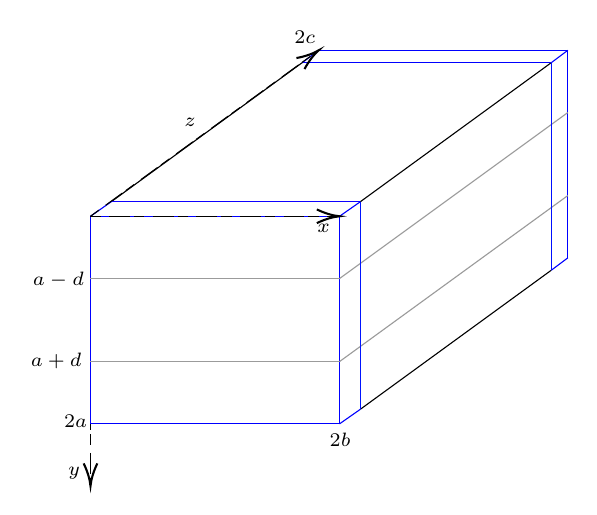
\begin{tikzpicture}[x=0.75pt,y=0.75pt,yscale=-1,xscale=1]
%uncomment if require: \path (0,461); %set diagram left start at 0, and has height of 461

%Straight Lines [id:da33793160626814234] 
\draw [color={rgb, 255:red, 0; green, 0; blue, 0 }  ,draw opacity=1 ] [dash pattern={on 3.75pt off 3pt on 7.5pt off 1.5pt}]  (60,120) -- (60,248) ;
\draw [shift={(60,250)}, rotate = 270] [color={rgb, 255:red, 0; green, 0; blue, 0 }  ,draw opacity=1 ][line width=0.75]    (10.93,-3.29) .. controls (6.95,-1.4) and (3.31,-0.3) .. (0,0) .. controls (3.31,0.3) and (6.95,1.4) .. (10.93,3.29)   ;
%Straight Lines [id:da21048665747646944] 
\draw    (70,113) -- (162,46) ;
%Straight Lines [id:da21496427185008327] 
\draw    (190,113) -- (282,46) ;
%Straight Lines [id:da04028217537075074] 
\draw [color={rgb, 255:red, 0; green, 0; blue, 255 }  ,draw opacity=1 ]   (60,120) -- (180,120) ;
%Straight Lines [id:da7170712168727287] 
\draw [color={rgb, 255:red, 0; green, 0; blue, 255 }  ,draw opacity=1 ]   (170,40) -- (290,40) ;
%Straight Lines [id:da12233767000161122] 
\draw [color={rgb, 255:red, 0; green, 0; blue, 255 }  ,draw opacity=1 ]   (60,220) -- (180,220) ;
%Straight Lines [id:da3869762813522424] 
\draw    (190,213) -- (282,146) ;
%Straight Lines [id:da05729970060070899] 
\draw [color={rgb, 255:red, 0; green, 0; blue, 255 }  ,draw opacity=1 ]   (60,120) -- (60,220) ;
%Straight Lines [id:da881902696420134] 
\draw [color={rgb, 255:red, 0; green, 0; blue, 255 }  ,draw opacity=1 ]   (180,120) -- (180,220) ;
%Straight Lines [id:da30748964416540847] 
\draw [color={rgb, 255:red, 0; green, 0; blue, 255 }  ,draw opacity=1 ]   (290,40) -- (290,140) ;
%Straight Lines [id:da4970694191237319] 
\draw [color={rgb, 255:red, 155; green, 155; blue, 155 }  ,draw opacity=1 ]   (60,150) -- (180,150) ;
%Straight Lines [id:da2761427702849881] 
\draw [color={rgb, 255:red, 155; green, 155; blue, 155 }  ,draw opacity=1 ]   (60,190) -- (180,190) ;
%Straight Lines [id:da8026720700371979] 
\draw [color={rgb, 255:red, 155; green, 155; blue, 155 }  ,draw opacity=1 ]   (180,190) -- (290,110) ;
%Straight Lines [id:da23722210789790243] 
\draw [color={rgb, 255:red, 155; green, 155; blue, 155 }  ,draw opacity=1 ]   (180,150) -- (290,70) ;
%Straight Lines [id:da9998354929478732] 
\draw [color={rgb, 255:red, 13; green, 0; blue, 255 }  ,draw opacity=1 ]   (70,113) -- (190,113) ;
%Straight Lines [id:da4132700627297399] 
\draw [color={rgb, 255:red, 0; green, 0; blue, 255 }  ,draw opacity=1 ]   (162,46) -- (282,46) ;
%Straight Lines [id:da5939794577660118] 
\draw [color={rgb, 255:red, 0; green, 20; blue, 255 }  ,draw opacity=1 ]   (190,113) -- (190,213) ;
%Straight Lines [id:da8623036562152813] 
\draw [color={rgb, 255:red, 0; green, 15; blue, 255 }  ,draw opacity=1 ]   (282,46) -- (282,146) ;
%Straight Lines [id:da8793888735498807] 
\draw [color={rgb, 255:red, 0; green, 0; blue, 255 }  ,draw opacity=1 ]   (180,120) -- (190,113) ;
%Straight Lines [id:da6169914746452605] 
\draw [color={rgb, 255:red, 0; green, 0; blue, 255 }  ,draw opacity=1 ]   (180,220) -- (190,213) ;
%Straight Lines [id:da8616702568255465] 
\draw [color={rgb, 255:red, 0; green, 0; blue, 255 }  ,draw opacity=1 ]   (60,120) -- (70,113) ;
%Straight Lines [id:da7336605374589271] 
\draw [color={rgb, 255:red, 0; green, 0; blue, 255 }  ,draw opacity=1 ]   (282,146) -- (290,140) ;
%Straight Lines [id:da4871143624254335] 
\draw [color={rgb, 255:red, 0; green, 0; blue, 255 }  ,draw opacity=1 ]   (282,46) -- (290,40) ;
%Straight Lines [id:da6094463937535262] 
\draw [color={rgb, 255:red, 0; green, 0; blue, 255 }  ,draw opacity=1 ]   (162,46) -- (170,40) ;
%Straight Lines [id:da8435206245989231] 
\draw [color={rgb, 255:red, 0; green, 0; blue, 0 }  ,draw opacity=1 ] [dash pattern={on 3.75pt off 3pt on 7.5pt off 1.5pt}]  (60,120) -- (178,120) ;
\draw [shift={(180,120)}, rotate = 180] [color={rgb, 255:red, 0; green, 0; blue, 0 }  ,draw opacity=1 ][line width=0.75]    (10.93,-3.29) .. controls (6.95,-1.4) and (3.31,-0.3) .. (0,0) .. controls (3.31,0.3) and (6.95,1.4) .. (10.93,3.29)   ;
%Straight Lines [id:da416605107929652] 
\draw [color={rgb, 255:red, 0; green, 0; blue, 0 }  ,draw opacity=1 ] [dash pattern={on 3.75pt off 3pt on 7.5pt off 1.5pt}]  (60,120) -- (168.38,41.18) ;
\draw [shift={(170,40)}, rotate = 143.97] [color={rgb, 255:red, 0; green, 0; blue, 0 }  ,draw opacity=1 ][line width=0.75]    (10.93,-3.29) .. controls (6.95,-1.4) and (3.31,-0.3) .. (0,0) .. controls (3.31,0.3) and (6.95,1.4) .. (10.93,3.29)   ;

% Text Node
\draw (168,122.4) node [anchor=north west][inner sep=0.75pt]  [font=\scriptsize]  {$x$};
% Text Node
\draw (48,239.4) node [anchor=north west][inner sep=0.75pt]  [font=\scriptsize]  {$y$};
% Text Node
\draw (104,71.4) node [anchor=north west][inner sep=0.75pt]  [font=\scriptsize]  {$z$};
% Text Node
\draw (46,214.4) node [anchor=north west][inner sep=0.75pt]  [font=\scriptsize]  {$2a$};
% Text Node
\draw (31,145.4) node [anchor=north west][inner sep=0.75pt]  [font=\scriptsize]  {$a-d$};
% Text Node
\draw (30,184.4) node [anchor=north west][inner sep=0.75pt]  [font=\scriptsize]  {$a+d$};
% Text Node
\draw (174,223.4) node [anchor=north west][inner sep=0.75pt]  [font=\scriptsize]  {$2b$};
% Text Node
\draw (157,29.4) node [anchor=north west][inner sep=0.75pt]  [font=\scriptsize]  {$2c$};


\end{tikzpicture}
      }

      \resizebox{0.8\textwidth}{!}
      { 
        

\tikzset{every picture/.style={line width=0.75pt}} %set default line width to 0.75pt        

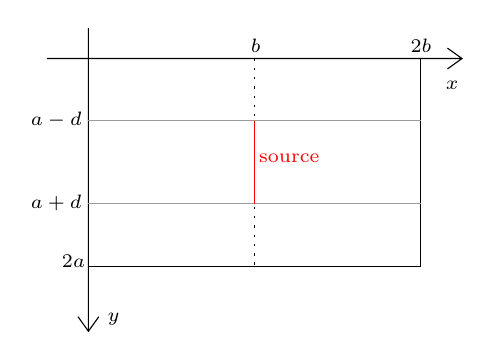
\begin{tikzpicture}[x=0.75pt,y=0.75pt,yscale=-1,xscale=1]
%uncomment if require: \path (0,300); %set diagram left start at 0, and has height of 300

%Straight Lines [id:da3480880018545507] 
\draw  [dash pattern={on 0.84pt off 2.51pt}]  (120,30) -- (120,130) ;
%Shape: Axis 2D [id:dp3637924149326488] 
\draw  (40,15.4) -- (40,161.4)(220,30) -- (20,30) (45,154.4) -- (40,161.4) -- (35,154.4) (213,25) -- (220,30) -- (213,35)  ;
%Shape: Rectangle [id:dp609433285561545] 
\draw   (40,30) -- (200,30) -- (200,130) -- (40,130) -- cycle ;
%Straight Lines [id:da15540762860028612] 
\draw [color={rgb, 255:red, 155; green, 155; blue, 155 }  ,draw opacity=1 ]   (40,60) -- (200,60) ;
%Straight Lines [id:da5236995862324196] 
\draw [color={rgb, 255:red, 155; green, 155; blue, 155 }  ,draw opacity=1 ]   (40,100) -- (200,100) ;
%Straight Lines [id:da00556491703537243] 
\draw [color={rgb, 255:red, 255; green, 0; blue, 0 }  ,draw opacity=1 ]   (120,60) -- (120,100) ;

% Text Node
\draw (211,39.4) node [anchor=north west][inner sep=0.75pt]  [font=\scriptsize]  {$x$};
% Text Node
\draw (48,151.4) node [anchor=north west][inner sep=0.75pt]  [font=\scriptsize]  {$y$};
% Text Node
\draw (194,19.4) node [anchor=north west][inner sep=0.75pt]  [font=\scriptsize]  {$2b$};
% Text Node
\draw (26,123.4) node [anchor=north west][inner sep=0.75pt]  [font=\scriptsize]  {$2a$};
% Text Node
\draw (117,19.4) node [anchor=north west][inner sep=0.75pt]  [font=\scriptsize]  {$b$};
% Text Node
\draw (11,54.4) node [anchor=north west][inner sep=0.75pt]  [font=\scriptsize]  {$a-d$};
% Text Node
\draw (11,94.4) node [anchor=north west][inner sep=0.75pt]  [font=\scriptsize]  {$a+d$};
% Text Node
\draw (121,75) node [anchor=north west][inner sep=0.75pt]  [font=\scriptsize,color={rgb, 255:red, 255; green, 0; blue, 0 }  ,opacity=1 ] [align=left] {source};


\end{tikzpicture}
        

% Pattern Info
 
\tikzset{
pattern size/.store in=\mcSize, 
pattern size = 5pt,
pattern thickness/.store in=\mcThickness, 
pattern thickness = 0.3pt,
pattern radius/.store in=\mcRadius, 
pattern radius = 1pt}
\makeatletter
\pgfutil@ifundefined{pgf@pattern@name@_64w1ndx3q}{
\pgfdeclarepatternformonly[\mcThickness,\mcSize]{_64w1ndx3q}
{\pgfqpoint{0pt}{-\mcThickness}}
{\pgfpoint{\mcSize}{\mcSize}}
{\pgfpoint{\mcSize}{\mcSize}}
{
\pgfsetcolor{\tikz@pattern@color}
\pgfsetlinewidth{\mcThickness}
\pgfpathmoveto{\pgfqpoint{0pt}{\mcSize}}
\pgfpathlineto{\pgfpoint{\mcSize+\mcThickness}{-\mcThickness}}
\pgfusepath{stroke}
}}
\makeatother

% Pattern Info
 
\tikzset{
pattern size/.store in=\mcSize, 
pattern size = 5pt,
pattern thickness/.store in=\mcThickness, 
pattern thickness = 0.3pt,
pattern radius/.store in=\mcRadius, 
pattern radius = 1pt}
\makeatletter
\pgfutil@ifundefined{pgf@pattern@name@_qnc3ayslt}{
\pgfdeclarepatternformonly[\mcThickness,\mcSize]{_qnc3ayslt}
{\pgfqpoint{0pt}{-\mcThickness}}
{\pgfpoint{\mcSize}{\mcSize}}
{\pgfpoint{\mcSize}{\mcSize}}
{
\pgfsetcolor{\tikz@pattern@color}
\pgfsetlinewidth{\mcThickness}
\pgfpathmoveto{\pgfqpoint{0pt}{\mcSize}}
\pgfpathlineto{\pgfpoint{\mcSize+\mcThickness}{-\mcThickness}}
\pgfusepath{stroke}
}}
\makeatother
\tikzset{every picture/.style={line width=0.75pt}} %set default line width to 0.75pt        

\begin{tikzpicture}[x=0.75pt,y=0.75pt,yscale=-1,xscale=1]
%uncomment if require: \path (0,300); %set diagram left start at 0, and has height of 300

%Shape: Rectangle [id:dp6810885499420589] 
\draw  [color={rgb, 255:red, 0; green, 0; blue, 255 }  ,draw opacity=1 ][pattern=_64w1ndx3q,pattern size=6pt,pattern thickness=0.75pt,pattern radius=0pt, pattern color={rgb, 255:red, 0; green, 0; blue, 255}] (180,30) -- (200,30) -- (200,130) -- (180,130) -- cycle ;
%Shape: Rectangle [id:dp9654892852591364] 
\draw  [color={rgb, 255:red, 0; green, 0; blue, 255 }  ,draw opacity=1 ][pattern=_qnc3ayslt,pattern size=6pt,pattern thickness=0.75pt,pattern radius=0pt, pattern color={rgb, 255:red, 0; green, 0; blue, 255}] (40,30) -- (60,30) -- (60,130) -- (40,130) -- cycle ;
%Straight Lines [id:da3480880018545507] 
\draw  [dash pattern={on 0.84pt off 2.51pt}]  (120,30) -- (120,130) ;
%Shape: Axis 2D [id:dp3637924149326488] 
\draw  (40,15.4) -- (40,161.4)(220,30) -- (20,30) (45,154.4) -- (40,161.4) -- (35,154.4) (213,25) -- (220,30) -- (213,35)  ;
%Shape: Rectangle [id:dp609433285561545] 
\draw   (40,30) -- (200,30) -- (200,130) -- (40,130) -- cycle ;
%Straight Lines [id:da15540762860028612] 
\draw [color={rgb, 255:red, 155; green, 155; blue, 155 }  ,draw opacity=1 ]   (40,60) -- (200,60) ;
%Straight Lines [id:da5236995862324196] 
\draw [color={rgb, 255:red, 155; green, 155; blue, 155 }  ,draw opacity=1 ]   (40,100) -- (200,100) ;
%Straight Lines [id:da00556491703537243] 
\draw [color={rgb, 255:red, 255; green, 0; blue, 0 }  ,draw opacity=1 ]   (120,60) -- (120,100) ;

% Text Node
\draw (211,39.4) node [anchor=north west][inner sep=0.75pt]  [font=\scriptsize]  {$z$};
% Text Node
\draw (48,151.4) node [anchor=north west][inner sep=0.75pt]  [font=\scriptsize]  {$y$};
% Text Node
\draw (194,19.4) node [anchor=north west][inner sep=0.75pt]  [font=\scriptsize]  {$2c$};
% Text Node
\draw (26,123.4) node [anchor=north west][inner sep=0.75pt]  [font=\scriptsize]  {$2a$};
% Text Node
\draw (117,19.4) node [anchor=north west][inner sep=0.75pt]  [font=\scriptsize]  {$c$};
% Text Node
\draw (11,54.4) node [anchor=north west][inner sep=0.75pt]  [font=\scriptsize]  {$a-d$};
% Text Node
\draw (11,94.4) node [anchor=north west][inner sep=0.75pt]  [font=\scriptsize]  {$a+d$};
% Text Node
\draw (121,75) node [anchor=north west][inner sep=0.75pt]  [font=\scriptsize,color={rgb, 255:red, 255; green, 0; blue, 0 }  ,opacity=1 ] [align=left] {source};
% Text Node
\draw (202,75) node [anchor=north west][inner sep=0.75pt]  [font=\scriptsize,color={rgb, 255:red, 0; green, 0; blue, 255 }  ,opacity=1 ] [align=left] {PML};
% Text Node
\draw (62,75) node [anchor=north west][inner sep=0.75pt]  [font=\scriptsize,color={rgb, 255:red, 0; green, 0; blue, 255 }  ,opacity=1 ] [align=left] {PML};


\end{tikzpicture}
      }
\end{frame}

\begin{frame}{Simulation Scenary}
    \begin{center}
      \resizebox{0.8\textwidth}{!}
      { 
        

\tikzset{every picture/.style={line width=0.75pt}} %set default line width to 0.75pt        

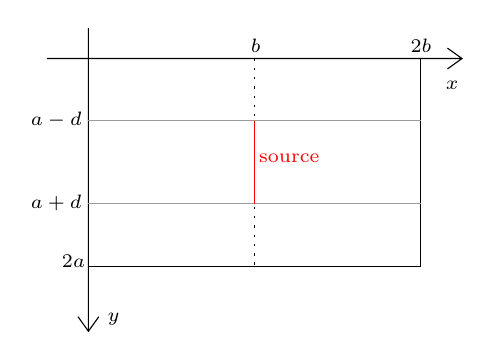
\begin{tikzpicture}[x=0.75pt,y=0.75pt,yscale=-1,xscale=1]
%uncomment if require: \path (0,300); %set diagram left start at 0, and has height of 300

%Straight Lines [id:da3480880018545507] 
\draw  [dash pattern={on 0.84pt off 2.51pt}]  (120,30) -- (120,130) ;
%Shape: Axis 2D [id:dp3637924149326488] 
\draw  (40,15.4) -- (40,161.4)(220,30) -- (20,30) (45,154.4) -- (40,161.4) -- (35,154.4) (213,25) -- (220,30) -- (213,35)  ;
%Shape: Rectangle [id:dp609433285561545] 
\draw   (40,30) -- (200,30) -- (200,130) -- (40,130) -- cycle ;
%Straight Lines [id:da15540762860028612] 
\draw [color={rgb, 255:red, 155; green, 155; blue, 155 }  ,draw opacity=1 ]   (40,60) -- (200,60) ;
%Straight Lines [id:da5236995862324196] 
\draw [color={rgb, 255:red, 155; green, 155; blue, 155 }  ,draw opacity=1 ]   (40,100) -- (200,100) ;
%Straight Lines [id:da00556491703537243] 
\draw [color={rgb, 255:red, 255; green, 0; blue, 0 }  ,draw opacity=1 ]   (120,60) -- (120,100) ;

% Text Node
\draw (211,39.4) node [anchor=north west][inner sep=0.75pt]  [font=\scriptsize]  {$x$};
% Text Node
\draw (48,151.4) node [anchor=north west][inner sep=0.75pt]  [font=\scriptsize]  {$y$};
% Text Node
\draw (194,19.4) node [anchor=north west][inner sep=0.75pt]  [font=\scriptsize]  {$2b$};
% Text Node
\draw (26,123.4) node [anchor=north west][inner sep=0.75pt]  [font=\scriptsize]  {$2a$};
% Text Node
\draw (117,19.4) node [anchor=north west][inner sep=0.75pt]  [font=\scriptsize]  {$b$};
% Text Node
\draw (11,54.4) node [anchor=north west][inner sep=0.75pt]  [font=\scriptsize]  {$a-d$};
% Text Node
\draw (11,94.4) node [anchor=north west][inner sep=0.75pt]  [font=\scriptsize]  {$a+d$};
% Text Node
\draw (121,75) node [anchor=north west][inner sep=0.75pt]  [font=\scriptsize,color={rgb, 255:red, 255; green, 0; blue, 0 }  ,opacity=1 ] [align=left] {source};


\end{tikzpicture}
        

% Pattern Info
 
\tikzset{
pattern size/.store in=\mcSize, 
pattern size = 5pt,
pattern thickness/.store in=\mcThickness, 
pattern thickness = 0.3pt,
pattern radius/.store in=\mcRadius, 
pattern radius = 1pt}
\makeatletter
\pgfutil@ifundefined{pgf@pattern@name@_64w1ndx3q}{
\pgfdeclarepatternformonly[\mcThickness,\mcSize]{_64w1ndx3q}
{\pgfqpoint{0pt}{-\mcThickness}}
{\pgfpoint{\mcSize}{\mcSize}}
{\pgfpoint{\mcSize}{\mcSize}}
{
\pgfsetcolor{\tikz@pattern@color}
\pgfsetlinewidth{\mcThickness}
\pgfpathmoveto{\pgfqpoint{0pt}{\mcSize}}
\pgfpathlineto{\pgfpoint{\mcSize+\mcThickness}{-\mcThickness}}
\pgfusepath{stroke}
}}
\makeatother

% Pattern Info
 
\tikzset{
pattern size/.store in=\mcSize, 
pattern size = 5pt,
pattern thickness/.store in=\mcThickness, 
pattern thickness = 0.3pt,
pattern radius/.store in=\mcRadius, 
pattern radius = 1pt}
\makeatletter
\pgfutil@ifundefined{pgf@pattern@name@_qnc3ayslt}{
\pgfdeclarepatternformonly[\mcThickness,\mcSize]{_qnc3ayslt}
{\pgfqpoint{0pt}{-\mcThickness}}
{\pgfpoint{\mcSize}{\mcSize}}
{\pgfpoint{\mcSize}{\mcSize}}
{
\pgfsetcolor{\tikz@pattern@color}
\pgfsetlinewidth{\mcThickness}
\pgfpathmoveto{\pgfqpoint{0pt}{\mcSize}}
\pgfpathlineto{\pgfpoint{\mcSize+\mcThickness}{-\mcThickness}}
\pgfusepath{stroke}
}}
\makeatother
\tikzset{every picture/.style={line width=0.75pt}} %set default line width to 0.75pt        

\begin{tikzpicture}[x=0.75pt,y=0.75pt,yscale=-1,xscale=1]
%uncomment if require: \path (0,300); %set diagram left start at 0, and has height of 300

%Shape: Rectangle [id:dp6810885499420589] 
\draw  [color={rgb, 255:red, 0; green, 0; blue, 255 }  ,draw opacity=1 ][pattern=_64w1ndx3q,pattern size=6pt,pattern thickness=0.75pt,pattern radius=0pt, pattern color={rgb, 255:red, 0; green, 0; blue, 255}] (180,30) -- (200,30) -- (200,130) -- (180,130) -- cycle ;
%Shape: Rectangle [id:dp9654892852591364] 
\draw  [color={rgb, 255:red, 0; green, 0; blue, 255 }  ,draw opacity=1 ][pattern=_qnc3ayslt,pattern size=6pt,pattern thickness=0.75pt,pattern radius=0pt, pattern color={rgb, 255:red, 0; green, 0; blue, 255}] (40,30) -- (60,30) -- (60,130) -- (40,130) -- cycle ;
%Straight Lines [id:da3480880018545507] 
\draw  [dash pattern={on 0.84pt off 2.51pt}]  (120,30) -- (120,130) ;
%Shape: Axis 2D [id:dp3637924149326488] 
\draw  (40,15.4) -- (40,161.4)(220,30) -- (20,30) (45,154.4) -- (40,161.4) -- (35,154.4) (213,25) -- (220,30) -- (213,35)  ;
%Shape: Rectangle [id:dp609433285561545] 
\draw   (40,30) -- (200,30) -- (200,130) -- (40,130) -- cycle ;
%Straight Lines [id:da15540762860028612] 
\draw [color={rgb, 255:red, 155; green, 155; blue, 155 }  ,draw opacity=1 ]   (40,60) -- (200,60) ;
%Straight Lines [id:da5236995862324196] 
\draw [color={rgb, 255:red, 155; green, 155; blue, 155 }  ,draw opacity=1 ]   (40,100) -- (200,100) ;
%Straight Lines [id:da00556491703537243] 
\draw [color={rgb, 255:red, 255; green, 0; blue, 0 }  ,draw opacity=1 ]   (120,60) -- (120,100) ;

% Text Node
\draw (211,39.4) node [anchor=north west][inner sep=0.75pt]  [font=\scriptsize]  {$z$};
% Text Node
\draw (48,151.4) node [anchor=north west][inner sep=0.75pt]  [font=\scriptsize]  {$y$};
% Text Node
\draw (194,19.4) node [anchor=north west][inner sep=0.75pt]  [font=\scriptsize]  {$2c$};
% Text Node
\draw (26,123.4) node [anchor=north west][inner sep=0.75pt]  [font=\scriptsize]  {$2a$};
% Text Node
\draw (117,19.4) node [anchor=north west][inner sep=0.75pt]  [font=\scriptsize]  {$c$};
% Text Node
\draw (11,54.4) node [anchor=north west][inner sep=0.75pt]  [font=\scriptsize]  {$a-d$};
% Text Node
\draw (11,94.4) node [anchor=north west][inner sep=0.75pt]  [font=\scriptsize]  {$a+d$};
% Text Node
\draw (121,75) node [anchor=north west][inner sep=0.75pt]  [font=\scriptsize,color={rgb, 255:red, 255; green, 0; blue, 0 }  ,opacity=1 ] [align=left] {source};
% Text Node
\draw (202,75) node [anchor=north west][inner sep=0.75pt]  [font=\scriptsize,color={rgb, 255:red, 0; green, 0; blue, 255 }  ,opacity=1 ] [align=left] {PML};
% Text Node
\draw (62,75) node [anchor=north west][inner sep=0.75pt]  [font=\scriptsize,color={rgb, 255:red, 0; green, 0; blue, 255 }  ,opacity=1 ] [align=left] {PML};


\end{tikzpicture}
      }
    \end{center}
      \begin{columns}
        
        \begin{column}{0.45\textwidth}
          \begin{table}[H]
          \resizebox{\textwidth}{!}
          {
            \begin{tabular}{|c|c|c|}
            \hline
            \textbf{Parameter} & \textbf{Description}               & \textbf{Value} \\ \hline
            $a$                & Half-length on $y$-axis              & 5 cm           \\ \hline
            $b$                & Half-length on $x$-axis              & 5 cm           \\ \hline
            $c$                & Half-length on $z$-axis              & 10 cm          \\ \hline
            $d$                & Half-distance between strips       & 2 cm           \\ \hline
            $N_x$              & Number of cells on $x$-axis          & 40             \\ \hline
            $N_y$              & Number of cells on $y$-axis          & 40             \\ \hline
            $N_z$              & Number of cells on $z$-axis          & 70             \\ \hline
            $N_{\textnormal{PML}}$          & Number of cells with PML on z-axis & 10             \\ \hline
            $\epsilon_{r_2}$          & Relative permittivity between strips & 5             \\ \hline
            \end{tabular}
          }
          \end{table}
          
        \end{column}

        \begin{column}{0.35\textwidth}
          \begin{table}[H]
          \resizebox{\textwidth}{!}
          {
            \begin{tabular}{|c|c|c|}
            \hline
            \textbf{Parameter}                           & \textbf{Description} & \textbf{Value} \\ \hline
            $N_x^c$                                      & Index centered on x  & 20             \\ \hline
            $N_y^c$                                      & Index centered on y  & 20             \\ \hline
            $N_z^c$                                      & Index centered on z  & 35             \\ \hline
            $N_{\textnormal{plate}}^{\textnormal{high}}$ & Y-index of top strip & 32             \\ \hline
            $N_{\textnormal{plate}}^{\textnormal{low}}$  & Y-index of low strip & 8              \\ \hline
            $\dx$                                        & ${2b}/{N_x}$         & 40             \\ \hline
            $\dy$                                        & ${2a}/{N_y}$         & 70             \\ \hline
            $\dz$                                        & ${2c}/{N_z}$         & 10             \\ \hline
            \end{tabular}
          }
          \end{table}
        \end{column}

      \end{columns}


\end{frame}

\begin{frame}{Boundary Conditions}
  \textbf{On Source} \\
  The source is located at $\pare{N_x^c, N_{\textnormal{plate}}^{\textnormal{low}} : N_{\textnormal{plate}}^{\textnormal{high}}, N_z^c}$. It will be considered that the source is on $\En_y$ as shown below: 

  \begin{figure}[H]
      \centering
      \includegraphics[width=0.45\textwidth]{../contents/input_source.png}
      \caption{Input electric field with frequency $f_c = \SI{3.0}{\giga\hertz}$, peak time $t_p = \SI{1.5}{\nano\second}$ and duration $t_f = \SI{5.0}{\nano\second}$. The Gaussian that limits the sine function has $\tau = \SI{0.5}{\nano\second}$.}
  \end{figure}
\end{frame}

\begin{frame}{Boundary Conditions}
  \textbf{On Conductor Strips} \\

  There is one strip located at $\pare{:, N_{\textnormal{plate}}^{\textnormal{low}}, :}$ and another at $\pare{:, N_{\textnormal{plate}}^{\textnormal{high}}, :}$. At these positions is valid:

  \begin{align}
      \En_x = \En_z = \Hht_y = 0
  \end{align}

  \textbf{Conductor Walls} \\

  The condition for conductor walls is the same as for conductor strips. Their positions are at: $\pare{0, :, :}$, $\pare{N_x-1, :, :}$, $\pare{:, 0, :}$,$\pare{:, N_y-1, :}$, $\pare{:, :, 0}$ and $\pare{:, :, N_z-1}$.
\end{frame}

\begin{frame}{Time Step}
  The time step was chosen to obey the Courant Stability condition:

  \begin{equation}
      \dt \leq \cfrac{1}{c_0\sqrt{\pare{\cfrac{1}{\dx}}^2 + \pare{\cfrac{1}{\dy}}^2 + \pare{\cfrac{1}{\dz}}^2}}
  \end{equation}
\end{frame}

\begin{frame}{Simulation Results}

  \begin{columns}
    
    \begin{column}{0.5\textwidth}
      
      \begin{figure}[H]
        \centering
        \includegraphics[width=\textwidth]{../contents/central_xy_plane.png}
        \caption{Central XY Plane.}
      \end{figure}

    \end{column}

    \begin{column}{0.5\textwidth}
      
      \begin{figure}[H]
        \centering
        \includegraphics[width=\textwidth]{../contents/central_zy_plane.png}
        \caption{Central ZY Plane.}
      \end{figure}

    \end{column}

  \end{columns}

\end{frame}

\section{Next Steps}
\begin{frame}{Next Steps}
  \begin{itemize}
    \item Choose indicators to measure performance of the developed codes,
    \item Deduce the equations for the proposed problem using Geometric Algebra,
    \item Implement the solution using Geometric Algebra in Python/Cython,
    \item Study the possibility to solve this type of problem with Quantum Computing.
  \end{itemize}
\end{frame}

\begin{frame}[allowframebreaks]
  \frametitle{References}
  \bibliographystyle{IEEEtran}
  \bibliography{../contents/bibliography.bib}
\end{frame}
\end{document}